\section*{Deep Learning Results}
Our model was able to classify the 12-classes (12 stimuli listed in \autoref{tab:stimuli_information}) with a 28.7\% accuracy rate (chance = 8.3\%) at a significance level of p=0.001. 
Significance values were determined by using the cumulative binomial distribution to estimate the likelihood of observing a given classification rate by chance. 
\autoref{fig:model_W_confusion} is a confusion matrix which shows the classification results for each stimulus.

%\vspace{-1em}
\begin{figure}[h] 
  \begin{center}
    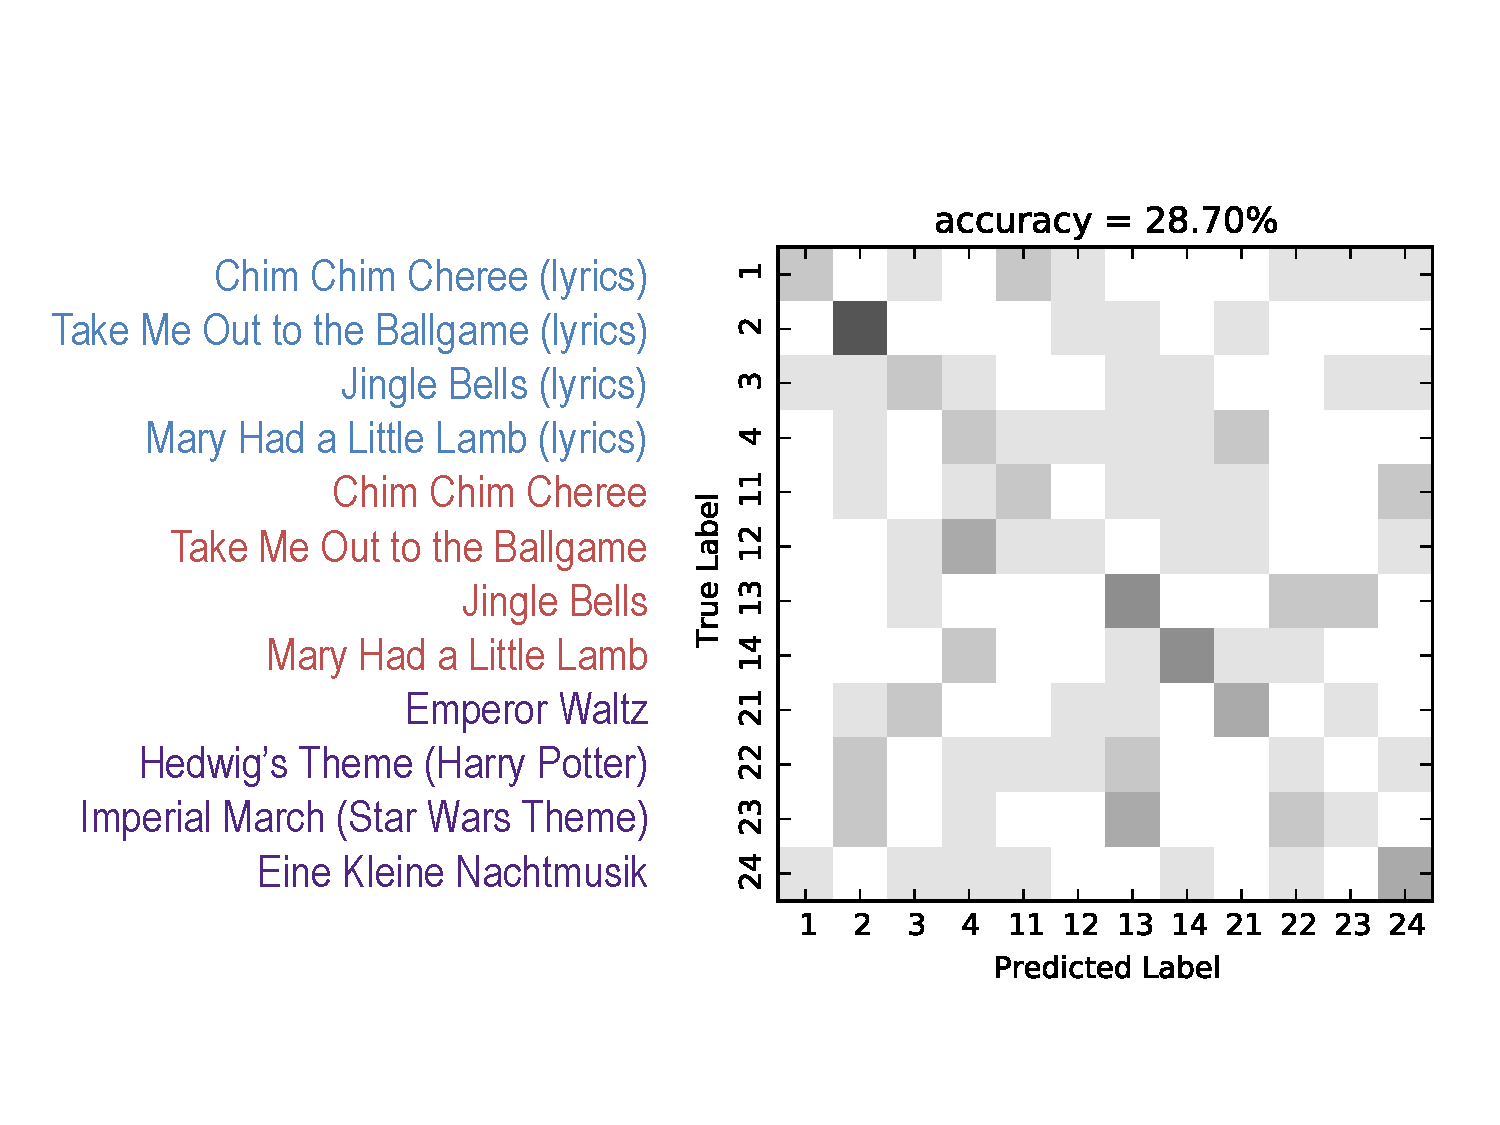
\includegraphics[width=.75\textwidth,keepaspectratio=true]{Figures/model_W_confusion}
   \\\vspace{-0.8em}
    \caption{12-class confusion matrix. Colour indicates the number of times each selection was made with darker colours indicating more selections.}
    \label{fig:model_W_confusion}
  \end{center}
%  \vspace{-1em}
\end{figure}

From the confusion matrix we can see that some stimuli are more accurately classified than others. 
Stimulus 2 is the most accurately classified. 
Stimuli 13 and 14 are also classified with some accuracy, and some confusion with their lyric counterparts (stimuli 3 and 4) can be seen.
Confusion between lyric and non-lyric pairs can also be seen with stimulus 1 being classified as stimulus 11.

\begin{figure}[h] 
  \begin{center}
    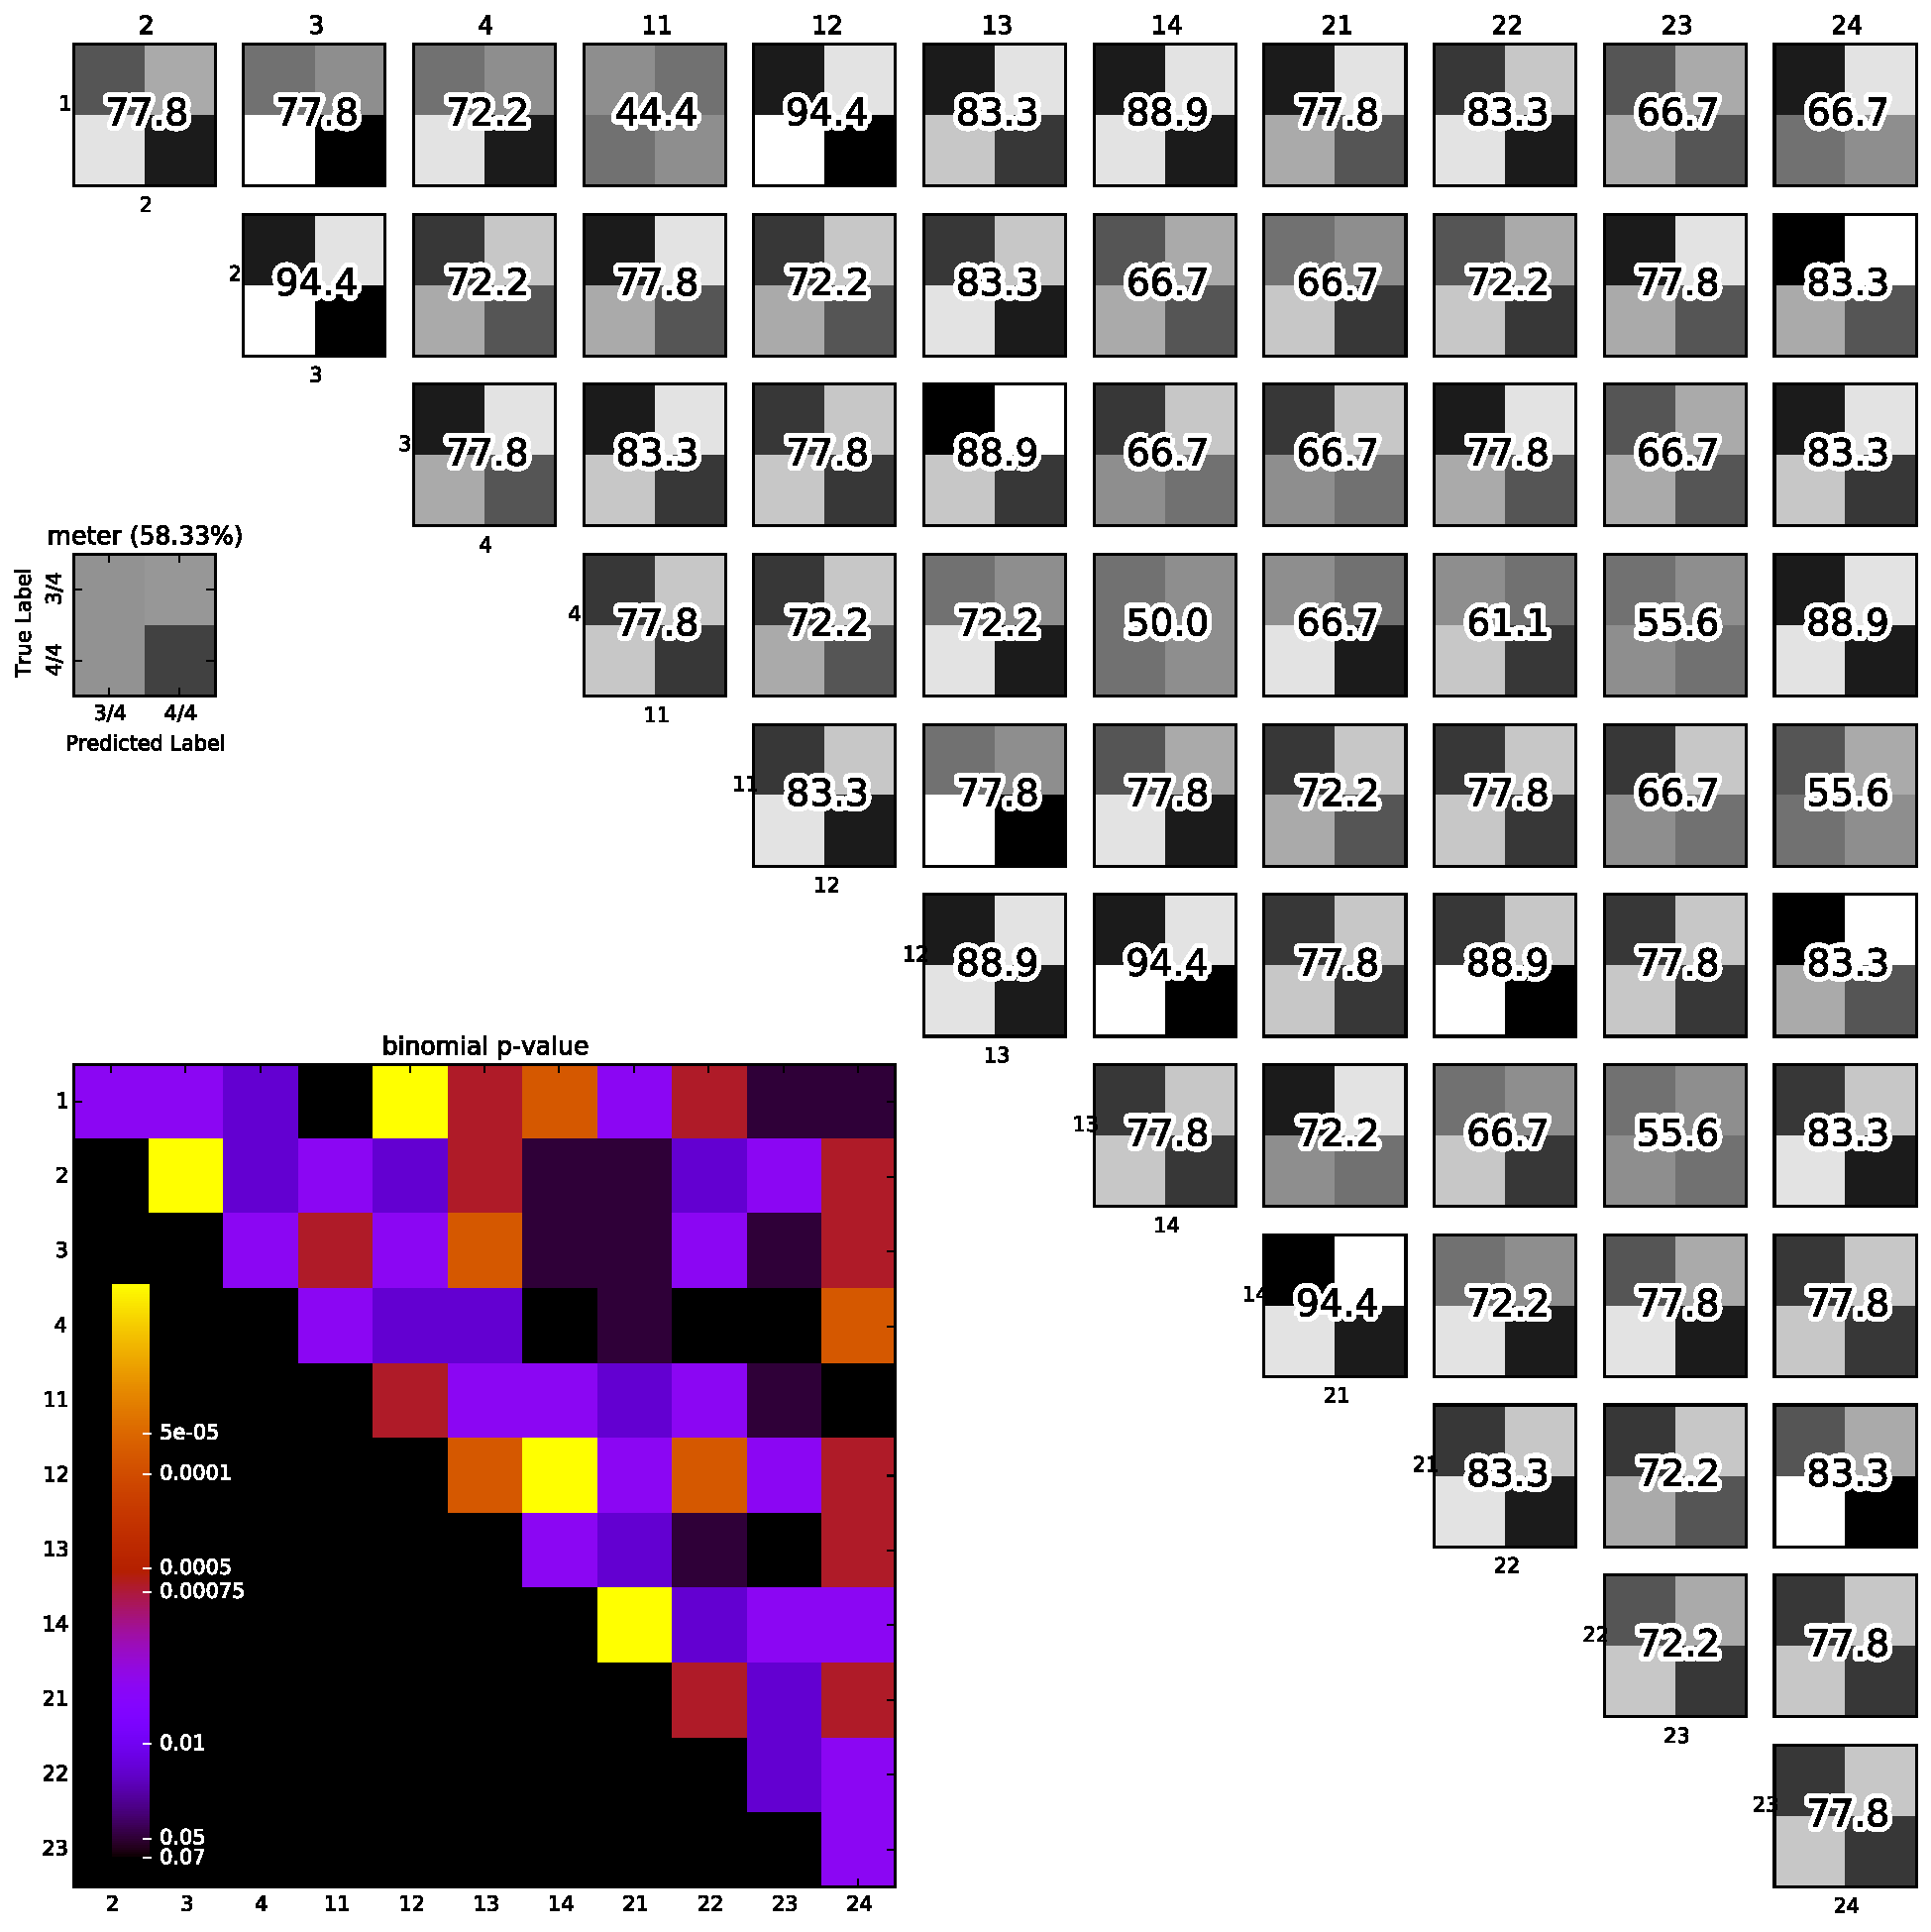
\includegraphics[width=.83\textwidth,keepaspectratio=true]{Figures/model_W_binary_confusion}
   \\\vspace{-0.8em}
    \caption{Binary confusion matrices.
    For each binary classification, only the 18 test trials belonging to either stimulus class A or stimulus class B were considered.
    The inset at the lower bottom visualizes the p-values determined by using the cumulative binomial distribution to estimate the likelihood of observing the respective binary classification rate by chance.}
    \label{fig:model_W_binary_confusion}
  \end{center}
  \vspace{-1em}
\end{figure}

To further investigate which pairs of stimuli our classifier can distinguish best we put all combinations of paired stimuli through our classifier.
This resulted in the series of binary confusion matrices in \autoref{fig:model_W_binary_confusion} that show us that some pairs of stimuli are more easily differentiated from each other than others. 
For example: Chim Chim Cheree with lyrics is classified correctly 100\% of the time when paired with Jingle Bells without lyrics. 
Within each binary confusion matrix chance is 50\%.
The statistical significance of each of the comparisons can be visualized in the figure's inset. 
Most of the binary comparisons are classified at a statistically significant level (p>0.05).